\documentclass[12pt]{article}
\usepackage{times}
\usepackage{graphicx}
\usepackage{cite}
\usepackage[margin=1in]{geometry}
\usepackage{bm}
\usepackage{cleveref}
\usepackage[font=small,labelfont=bf]{caption}
\usepackage{subcaption}
\captionsetup[subfigure]{subrefformat=simple,labelformat=simple}
\renewcommand\thesubfigure{(\alph{subfigure})}
\geometry{a4paper}
\usepackage{float}
%\usepackage{cite}
\newcommand{\beginsupplement}{%
  \setcounter{table}{0}
  \renewcommand{\thetable}{S\arabic{table}}%
  \setcounter{figure}{0}
  \renewcommand{\thefigure}{S\arabic{figure}}%
}
\usepackage{array}
\newcolumntype{L}[1]{>{\raggedright\let\newline\\\arraybackslash\hspace{0pt}}m{#1}}
\newcolumntype{C}[1]{>{\centering\let\newline\\\arraybackslash\hspace{0pt}}m{#1}}
\newcolumntype{R}[1]{>{\raggedleft\let\newline\\\arraybackslash\hspace{0pt}}m{#1}}

\begin{document}

\title{A versatile method for simulating the dynamic mechanical structure of cytoskeletal networks}
\author{Simon L. Freedman, Shiladitya Banerjee, Glen M. Hocky, Aaron R. Dinner}
\date{}
\maketitle
\begin{abstract}
  The cooperative mechanics of filamentous actin and myosin in the cytoskeleton comprise one of three active polymer
  networks that give the cell its shape, size, and motion. We have developed a computational model to study this network that incorporates 
  the mechanical interactions of actin filaments, actin crosslinkers, and myosin motors to further
  probe their behavior in a disordered ensemble, such as in vitro reconstitutions that mimic the cytoskeleton of non-muscle cells. 
  We will show that this model can reproduce the underlying mechanisms of reorganization
  present in crosslinked actomyosin networks. We benchmark this model against well established experimental results regarding fluctuations of
  semiflexible polymers, rheology of crosslinked actin networks, and actomyosin interactivity in sliding filament assays. 
\end{abstract}
\section{Introduction} 
The collective activity of many-particle systems where pair-wise particle interactions are well understood 
can be eluicidated via molecular dynamics simulations. 
A biomolecular example involves the proteins actin and myosin in the cytoskeleton of non-muscle cells. In that
environment, actin monomers polymerize into polar actin filaments (F-actin) which are microns long and
nanometers thick, and myosin motor proteins aggregate onto $0.4\mu m$ long backbones to form myosin minifilaments \cite{niederman1975}. 
For precessive motors, such as myosin II, the binding of myosin to actin, followed by ATP hydrolosis and subsequent
unbinding, results in the relative motion of myosin with
respect to actin toward the positive (barbed) end of an actin filament. In the cytoskeleton, this
motion drives many biological processes, including endocytosis, cell-division and maintenance of cell shape
\cite{stricker2010, murrell2012}.
\par
The mechanism through which myosin can walk on actin has been extensively studied in muscle cells, where actin
filaments are arranged in parallel bundles called sarcomeres. A myosin filament binds to two antipolar
sarcomeres, walks toward the barbed end of both, and the tension along the myosin pulls the 
sarcomeres together, resulting in muscle contraction\cite{huxley1969}. 
However, in the cytoskeleton of nonmuscle cells, there is no inherent ordering of actin or myosin filaments, so while
interactions between individual myosin and actin filaments exist, how 
they act in concert to produce a variety of behaviors is an active area of research 
that coule be further elucidated with an accurate computational model of the system\cite{murrell2012, stam2015, murrell2015}. 
\par
The goal of this work is to present a mathematical model, in the form of a non-equilibrium molecular dynamics
simulation, that can efficiently explore the structural and dynamical phase space of 
disordered ensembles of semiflexible filaments, molecular motors, and crosslinking proteins.
This mathematical model can guide our understanding of the relationship between
the microscopic biochemical protein-protein interactions and the macroscopic mechanical functionality of the ensemble. Additionally,
because the model simulates filaments, motors, and crosslinkers in space and time, it will enable us to learn the trajectory
of an ensemble, and how intermediate mesoscopic structures tune network functionality.
\par
The key achievements of this model are that it is well bench-marked to reproduce known experimental results for actin
filaments, ensembles of actin and crosslinkers (passive networks), and ensembles of actin and myosin 
(active networks). 
At the polymer level, we will reproduce predicted spatio-temporal fluctuations of actin filaments. 
For passive crosslinked networks we will reproduce known stress strain
relationships. For active networks, we will reproduce well-understood velocity distributions of actin
filaments in a myosin motility assay. Separately, we use the simulation to demonstrate how disordered ensembles of 
actin filaments and crosslinkers can be rearranged by myosin motors to form tunable structures with distinct biophysical and
mechanical functionality\cite{freedman2016}.  
\par
While our simulation is primarily motivated by \textit{in vitro} and \textit{in vivo} experiments, the implementation 
has been influenced by several other computational models of actin and myosin. 
We briefly review these various computational models to show how other models have
influenced ours, and where we differ.
Most prominently, a number of publications have dealt with understanding the rheological properties of crosslinked actin
networks\cite{mackintosh1995, head2003, wilhelm2003, kim2009}.  
For example, to study the viscoelasticity of passive networks,  Head, et al., simulated distributed actin filaments randomly 
on a $2D$ plane, crosslinked filament intersections to form a force-propogating network, sheared 
this network and let it relax to a minimum energy, corresponding to a chemical equilibrium \cite{head2003}. 
From this model, they were able to identify three elastic regimes,
characterized by the mean distance between crosslinkers and the temperature. 
Dasanyake, et. al., extended this model to include a term in the potential energy that corresponded to
myosin motor activity, and observed the emergence of force chains that tramsmit stress throughout the network,
which could help understand how contractile stress can emerge from a disordered network \cite{dasanyake2011}.
These models predict the mechanical equilibrium behavior of the actin / crosslinker and the actin / myosin
systems; i.e., at a particular time, they answer questions such as, how well can this cytoskeletal network propogate
force, and how can crosslinker concentrations alter mesh stiffness.
\par
Other simulations focus on the ensemble motion of a myosin minifilament with respect to a single actin filament.  
Erdmann and Schwarz used Monte Carlo simulations to verify a master equation that expresses the probability that $N$ motors are 
bound at time $t$ to a single filament\cite{erdmann2012}. Based on this model they are able to make accurate predictions for 
the duty ratio and force velocity curves for myosin. Stam et al. used simulations to study force buildup on a single 
filament by a multi-headed motor and found
distinct timescale regimes over which different biological motors could exert force and act as crosslinkers
\cite{stam2015}. These models of actin-myosin interaction are important to understand the mechanics at
the level of a single filament, and their results can be incorporated into larger network simulations. 
\par
Wang and Wolynes \cite{wang2012} model the F-actin networks as a graph of crosslinkers (nodes) and rigid actin filaments
(edges) in which myosin motor activity is simulated via antisymmetric kicks along the filaments. Their results include a
binary phase diagram of networks which are either contractile or not as a function of cross linker and myosin
densities. While the simplicity of their model is intriguing, their simulation does not account for filament bending, 
and their integration is performed via Monte Carlo, and is thus more applicable to structure formation than dynamics.
Nedelec performs dynamic simulations of ensembles of semiflexible microtubules and kinesin motor proteins
which have many of the same properties as actomyosin networks and uses them to explore aster and network formation in microtubule
assays \cite{nedelec2007} and has recently shown their applicability to actin networks \cite{ennomani2016}.
Gordon et al. \cite{gordon2012} and Kim \cite{kim2014} similarly simulate dynamics of F-actin networks and include
semiflexible filaments, motors and cross linking proteins. Gordon succeeded in showing various structures that can emerge
from assemblies of this type and Kim shows how changing concentrations of cross linker and motor densities can alter how
much force is generated by the network.
\par
Our model is constructed by including many of the best features of these preceding models.
We will use the potential energy for an actin filament as described by Head et al., for simulating actin filaments that can 
both bend and stretch with slight differences in how we actually simulated 
internal forces on filaments. In contrast to references \cite{head2003, dasanyake2011}, we will 
simulate non-equilibrium dynamics, including fluctuations due to non-zero temperature,  
crosslinkers and myosins binding and unbinding, and the precessive activity of myosin.  
Force propagation rules and binding kinetic equations will be similar to those of
\cite{nedelec2007, gordon2012}. Our simulations will be most similar to those
performed in references \cite{kim2014, ennomani2016} and we hope to expand on
their methods of exploring actomyosin via agent based molecular dynamics by
showing how they can shed light on a variety of systems of current experimental interest.
\section{Model}  
In the interest of computational efficiency we have chosen to coarse grain actin filaments, myosin minifilaments, and
crosslinker proteins at length scales relevant for network behavior. Actin filaments are
modeled as polar worm-like chains (WLC) such that one end of the WLC represents the barbed end of a filament and the
other end of the filament represents its pointed end.  
Crosslinkers are modeled as Hookean springs such
that both ends of the spring (heads) can bind and unbind from filaments. Thus, crosslinkers can increase network connectivity
which is understood to increase the length-scale of network contraction \cite{murrell2015} and bundle actin filaments
into force propogating chains as observed in experiment \cite{gardel2004, murrell2012, murrell2014, freedman2016}. 
Molecular motors are modeled as crosslinkers such
that a head bound to a filament will walk toward the filament's barbed end. Thus motors can slide filaments,
translocate across filaments, and increase network connectivity, which are instrumental mechanisms when determining
network behavior\cite{murrell2014}. We chose to parameterize our model in $2D$ as the in vitro experiments we wish to
interpret are relatively flat and
approximating the system as $2D$ allows us to simulate larger systems for longer times. Because we use a $2D$ system to
represent a $3D$ experiment, we exclude steric interaction for our filaments and crosslinkers, to account for
some of the freedom lost from the reduction in dimensionality. This implementation of filaments, motors and crosslinkers allows for 
motor-driven filament sliding and filament buckling, as seen in \Cref{fig:toys},
both of which are instrumental for actomyosin contractility \cite{murrell2012}.
\begin{figure}[H]  
  \centering
  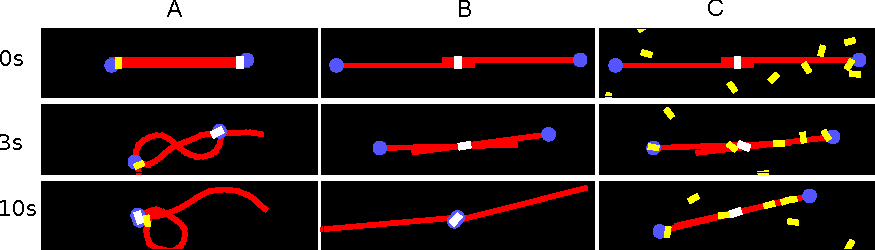
\includegraphics[width=\textwidth]{figs/minimal.pdf}
  \caption{
  \label{fig:toys}%
  Time series of three antiparallel $10\mu m$ filaments (red) interacting with a
  minimal set of motors (white) and crosslinkers (yellow) for $10s$. Barbed ends
  of filaments are marked by a blue dot.  
  (A) Filaments are semiflexible ($21$ bead-spring chain) and pinned on the left
  by a crosslinker, so the motor-filament interaction yields contraction via buckling. 
  (B) Filaments are rigid ($2$-bead-spring chains) and unpinned, so 
  motor-filament interaction yields unimpeded sliding of filaments. As a result,
  they transition from an initially extended state, to a contracted state
  at $t=3s$ and back to a fully extended polarity sorted state at $t=10s$.
  (C) Filaments and motor are the same as (B) but with a population of
crosslinkers near the filaments that arrests the filaments in a contracted state. } 
\end{figure}
\subsection{Worm-like chain semiflexible filaments}
The WLC model for actin filaments is implemented as a bead spring chain with $N+1$ beads connected by $N$ harmonic
springs (links) and $N-1$ angular harmonic springs, as depicted in \Cref{fig:filament}(A). The linear springs 
penalize stretching, and keep the filament's average end to end length constant, and the $N-1$ angular harmonic springs
penalize bending and maintain a constant persistence length for free filaments. 
The internal forces on actin filaments can be obtained from the gradient of the potential energy $U_f$
\begin{eqnarray}
  U_f &=& U_{stretch} + U_{bend}\\
  U_{stretch}&=&{k_a\over2}\sum_{i=1}^{N}{(|d_i| - l_a)^2}\\\nonumber
  U_{bend}&=&{\kappa_B\over 2l_a}\sum_{i=2}^N{\theta_i^2}\\\nonumber
  \label{eqn:Ufil}
\end{eqnarray}
where $d_i = r_i-r_{i-1}$, $\theta_i = \arccos{\left({d_i\cdot d_{i-1}\over |d_i||d_{i-1}|}\right)}$, $k_a$ is the
stretching force constant, $\kappa_B$ is the bending modulus, and $l_a$ is the equilibrium length of a
link. 
\par
For a confined semiflexible filament, it has been shown that for a polymer of a
given persistence length $L_p$, the shortest length that should be considered as
unbending ($l_a$) is given by $l_a\approx A^{2/3}L_p^{1/3}$ where $A$ is a
length scale associated with the confinement of the
filament \cite{odijk1983}. In these simulations, filaments were confined by
nearby motors and crosslinkers. Since the smallest motor or crosslinker density
used was $\rho_m=0.1\mu m^{-2}$, $A\ge1/\sqrt{0.1\mu m^{-2}}\Rightarrow l_a\ge5\mu m$.
In general, we used $l_a=1\mu m$. 
\par
The bending force constant is derived from the persistence length $L_p$ such that
$\kappa_B = L_p k_B T$ where $k_B$ is Boltzmann's constant and $T$ is the temperature \cite{rubinstein}.
Experimentally, the stretching force constant has been measured $k_a=40-70pN/nm$ \cite{kojima1994, higuchi1995};
however, simulating a network of filaments with this large of a stiffness would
have been computationally infeasible since the maximum timestep of a simulation is inversely
proportional to the largest stiffness in the simulation. Therefore, we set ${\kappa_B\over l_a} <<k_a$, so that the filaments
were much easier to bend than to stretch, enabling us to run network sized 
simulations. We verified that $k_a$ did not effect the persistence length of the
filament, as seen in the Supplement.
\subsection{Dynamic Hookean crosslinkers}
Within the cytoskeleton, various actin binding proteins, known as crosslinkers 
bind and unbind from actin filaments, thereby propogating force from one to
another. Thus, model crosslinkers must be able to attach and detach from actin filaments,
and be compliant in order to propagate force. They are modeled as Hookean springs, with stiffness
$k_{cl}$ and rest length $l_{cl}$. Like actin filaments, the Young's modulus of
most crosslinkers is significantly higher than would be reasonable to simulate; 
therefore, for network simulations without large external forces, we set $k_{cl}=k_a$ 
so that the bending mode of actin filaments was signicantly softer than the stretching mode of
crosslinkers. Their rest length $l_{cl}$ corresponds to the size of the crosslinker
and therefore will differ based on the particular actin-binding protein one wishes to simulate. 
For example, for fascin, $l_{cl}\approx10nm$ and for filament, $l_{cl}\approx150 nm$.
\par
At each time step of the simulation an unattached crosslinker head is allowed to attach to nearby
filaments and an attached crosslinker head can detach. 
The probability of a head attaching to an actin filament is a Gaussian distributed random variable, such that
\begin{equation}
  P_{cl}^{on} = k_{cl}^{on}dt\exp(-r^2/R^2)
  \label{eqn:cl_on}
\end{equation} 
where $r$ is the shortest distance from the head to the actin filament and $R = \sqrt{2k_B T\over k_{cl}}$ 
where $k_B$ is Boltzmann's constant and $T$ is the temperature. 
For crosslinker detachment we assume that the behavior is that of a slip bond with Bell's law behavior, 
such that a higher
tensile force along the crosslinker backbone will result in a higher probability of detachment\cite{bell1978}. Thus, 
\begin{equation}
  P_{cl}^{off} = k_{cl}^{off} dt\exp{\left(  F x_{cl}/k_B T\right)}  
  \label{eqn:cl_off}
\end{equation}
where $F$ is the force along the crosslinker backbone, and $x_{cl}$ is a characteristic bond length \cite{stam2015}. 
\par
When a crosslinker is bound to a filaments at both ends, it will necessarily be stretched or compressed. 
If it were allowed to relax independently of the actin filaments to which it is bound. 
it would no longer lie on those filaments. Therefore, the tensile force stored on a stretched or compressed
crosslinker is propagated onto those actin filaments via the lever rule outlined in 
\cite{nedelec2002, gordon2012}. Specifically, if the tensile force of a crosslinker at point $r_j$ between 
filament beads $i$ and $i+1$ is $F_{cl}$, then, 
\begin{eqnarray} 
  F_i &=& F_{cl}\left|\left( {r_j - r_i \over r_{i+1} - r_i }\right)\right|\\\nonumber
  F_{i+1} &=& F-F_i 
  \label{eqn:lever}
\end{eqnarray}
will be the forces on beads $i$ and $i+1$ respectively due to the crosslinker.
\subsection{Active crosslinking motors}
Within the cytoskeleton, tens of myosin II motors aggregate into bipolar ensembles called myosin minifilaments
\cite{stam2015}. While the mechanochemical process through which individual myosin motors walk along actin filaments is complex, 
motility assay experiments have shown that on average bound myosin II heads walk at an unloaded speed of $v_0\approx1\mu m/s$ along actin
filaments\cite{finer1994}. To a first approximation, minifilaments therefore should also 
have a mean speed of $1\mu m/s$ (although see \cite{stam2015} and \cite{walcott2012} for higher order measurements). 
Since myosin also functions to increase the local elasticity of networks wherever it is bound, the myosin is modeled
similarly to a crosslinker, in that it behaves like a Hookean spring with two heads, a stiffness $k_{m}$ and a rest
length $l_m$. It should be noted, however, that the two heads of this spring do not correspond directly to individual
molecular myosin heads; rather each of them represents tens of myosin molecules, and their rate constants will reflect
that notion. 
It would be undesirable for a myosin minifilament to stretch, 
since experimentally they have a very high
Young's modulus and it is unlikely that their length would change noticably in the cytoskeleton. 
Thus we set $k_m=k_a$ so that the bending of actin is still the softest mode. 
The rest length was set to the average length of minifilaments, $l_m=0.5\mu m$\cite{niederman1975}.
Attachment and detachment kinetics for motors are the same as for crosslinkers, subscripted with $m$
instead of $cl$ in \Cref{eqn:cl_on,eqn:cl_off}. One extra parameter is needed $k_m^{end}$ for the
detachment of myosin from the barbed end of a filament, as detachment from the end is significantly more probable than
from the rest of the filament.
Similarly, force propogation onto minifilaments is done using the lever rule described in \Cref{eqn:lever}.
\par
Unlike crosslinkers, motors precess towards the barbed end of actin filaments to which they are bound 
at speeds that linearly decrease with tensile force along the motor. 
The motor head therefore is fastest if the minifilament is
compressed (pre-powerstroke) and slowest if the minifilament is stretched (post powerstroke) 
going to $0$ when the force on the minifilament is the stall force $F_s\approx 3.85pN$ \cite{nedelec2002, gordon2012}; i.e.,  
\begin{equation} 
  v(F_{||}) = v_0\left( 1-{F_{||}\over F_s} \right)
    \label{eqn:myo_vel}
\end{equation} 
where $F_{||}$ is the force on the motor, projected along the tangent vector of the
actin filaments.
The minor differences between crosslinkers and motors allow us treat them equivalently, by 
setting $v_0 = 0$ for the crosslinkers.  
\subsection{Dynamics}
We use overdamped Langevin dynamics to solve for the motion of actin filaments, myosin minifilaments and crosslinkers.
The Langevin equations of motion for a spherical bead of
mass $m$, radius $R$ at position $r(t)$ at time $t$, being forced by an external force $F(t)$ is
\begin{equation}
  m\ddot{r}(t) = F(t) + B(t) - 4\pi R\nu \dot{r}(t)
  \label{eqn:lang}
\end{equation} 
where $B(t)$ is Brownian forcing term, to simulate a temperature, $\nu$ is the dynamic viscosity of the bead's
environment, and we have used the Einstein relation for the damping term.  
Since the fastest motion in this simulation is that of the myosin, and a $0.4\mu m$ myosin minifilament moving at
a speed of $1\mu m/s$ in a liquid at least as viscous as water ($\nu_D=10^6\mu m^2/s$ dynamic viscosity) has a very low Reynold's
number ($Re \approx 4*10^{-7}$) we assume the dynamics are overdamped and set $m=0$ in \Cref{eqn:lang}.
Furthermore, in the limit of small $\Delta t$, we may write $\dot{r(t)} \approx {r(t+\Delta t)-r(t)\over \Delta t}$. These two
approximations allow us to rewrite \Cref{eqn:lang} as 
\begin{equation}  
  r(t+\Delta t) = r(t) + F(t)\mu \Delta t + B(t) \mu \Delta t
  \label{eqn:overdamped}
\end{equation}
where $\mu = (4\pi R\nu)^{-1}$. For the brownian term, we use the form of Leimkuhler and Matthews \cite{leimkuhler2013} that has
been shown to minimize deviations from canonical averages in harmonic systems,
\begin{equation}
  B(t)=\sqrt{2k_BT\over\mu \Delta t}\left({W(t)+W(t-\Delta t)\over2}\right)
  \label{eqn:baoab_brownian}
\end{equation} 
where $W(t)$ is a Wiener process, in this case a random number drawn from the normal distribution $N(0,1)$. 
\subsection{Environment}
\par
Because the probability of motor attachment drops off exponentially as the distance squared from a filament, it is
highly inefficient to check for motor attachment for every filament in the simulation. Rather, a cutoff distance
$r_c>3R/2$ (where $R$ is defined above for \Cref{eqn:cl_on})
is determined such that if the distance between a motor and a filament is greater than $r_c$ the probability of
attachment is assumed to be $0$. A grid of lattice size $2r_c$ is drawn on the
$2D$ plane of the simulation, and the position of a filament is approximated as the points on the grid nearest to the
beads of the filament. Thus, to determine if a motor will bind to a filament at time $t$, it is sufficient to
only attempt attachment to filaments that are indexed at the four nearest grid points to a motor. 
\par
In general we use periodic boundary conditions so as to limit effects of a boundary and to mimic a system larger than
the one we simulate. Rigid boundaries as well as Lees-Edwards boundaries for shearing simulations have also been
implemented. The value for $\Delta t$ in \Cref{eqn:overdamped} generally depends on both the unloaded myosin speed
$v_0$ and the largest stiffness in the simulation $k_f$. For $k_f = 10pN/\mu m$ and $v_0=1\mu m/s$ a value of $\Delta t =
0.00001 s$ was low enough to iteratively solve \Cref{eqn:overdamped} without accumulating large error. 
The length and width of the simulations were chosen so as to be high enough to avoid boundary artifacts. 
A complete list of simulation parameters chose for each experiment can be seen in the Supplement
\section{Results}
\subsection{Actin Filaments Exhibit Predicted Spatial and Temporal Fluctuations}
For a two dimensional filament composed of links $d_1\cdots d_N$ with a constant link length $l_a$, constant total contour
length $L$, and where a small bend of link
$d_i$ with respect to link $d_{i-1}$ will result in a local change in free energy of ${\kappa_B\over2l_a\theta_i^2}$, it
is possible to show explicitly that \cite{frontali1979}
\begin{equation}
  \langle\theta^2(l)\rangle = {l_a\over L_p}
  \label{eqn:thsq}
\end{equation}
\begin{equation} 
  \langle\cos(\theta(l))\rangle = \exp{(-l_a/2L_p)}
  \label{eqn:costh}
\end{equation} 
where $\theta(l) = \theta_j - \theta_i$ $(1<i<j\le N)$, $l = l_a(j-i)$ and $L_p$ is the persistence length. 
To test our WLC model against these predictions, we let $100$ filaments of $L=200\mu m$ and $\kappa_B=0.08 pN\mu m^2$ fluctuate at
$T=300K$ for $T_f = 100s$ and measured the resulting filament configuration every $1s$, as that was more than enough
time for configurations to decorrelate. The first $10$ seconds of each simulation was disregarded as filaments had not
yet equilibrated, and the first and last $25\mu m$ of each filament were disregarded because of possible boundary
effects. 
For each of the $90000$ filament configurations, and for each $l\in{0,1,2,..,150}\mu m$,
$\theta^2(l)$ and $\cos(\theta(l))$ were calculated, and their respective averages are plotted in 
\Cref{fig:filament}(B), along with the expected behavior given the input $\kappa_B$.  
Further measurements of the persistence length as well as verifications of its independence on
other filament parameters is available in the supplement.
\par
Another benchmark for semiflexible filaments were the temporal fluctuations of a semiflexible filament.
Fluctuations transverse to the filament orientation have been 
shown to increase as $\langle dr_{\perp}^2\rangle\propto t^{3/4}$ while 
longitudinal fluctuations have been shown to increase as
$\langle dr_{||}^2\rangle\propto t^{7/8}$ \cite{everaers1999}. To tests these predictions, we followed the procedure outlined in
\cite{everaers1999} and generated $N = 100$ initial filament configurations of a $20\mu m$ filament. For each configuration
we ran $M = 100$ simulations of the filament fluctuating for $1s$. At each timestep each of the two ends of the
filament thus had $M$ possible position $r_e(t)$. For each of these clouds of points
shown in \Cref{fig:filament}C, we calculated the moments, as the eigenvalues of 
the covariance matrix $cov(r_e(t)\cdot \hat{i},r_e(t)\cdot \hat{j})$ where
$i,j\in\{x,y\}$.
The larger eigenvalue $\lambda_1(t)$ corresponds to the transverse fluctuations
(i.e., $\lambda_1(t)\propto t^{3/4}$) while the smaller eigenvalue corresponded to 
longitudinal fluctuations ($\lambda_2(t)\propto t^{3/4}$). We show these results
in \Cref{fig:filament}D. Each data point is the average over the $2N$ eigenvalues
for $\lambda_1(t)$ and $\lambda_2(t)$ while the error bars are the standard deviations for the
distribution of these values. As seen, they are in good agreement with the predicted behavior. 
\begin{figure}[H] 
  \centering
  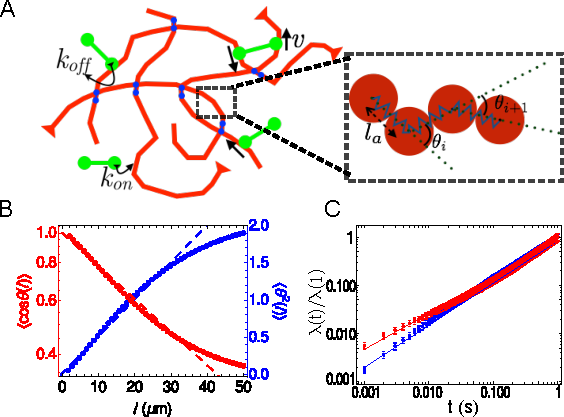
\includegraphics[scale=1.2]{figs/filament/pl_fig.pdf}
  \caption{\label{fig:filament}
  Actin filament diagram and fluctuations.
  (A) Sketch of the bead spring chain, illustrating the model.
  (B) Decorrelation of tangent vectors (red dots) and fluctuations in angles between links (blue dots) 
  as a function of the arc length between them. Dashed lines show expected behavior 
  for $\kappa_B=0.08 pN\mu m^2$.
  (C) Gray dots show positions of the end points of the filament at different times.
  Red arrow marks the larger eigenvalue of the covariance matrix of the positions
  of the endpoints (transverse fluctuations) while the blue arrow shows the longitudinal
  fluctuations. 
  (D) Eigenvalues of covariance matrices for the positions of endpoints of filaments as a function of time.  
  Red dashed line is $t^{3/4}$ and blue dashed line is $t^{7/8}$ as predicted by \cite{everaers1999}. 
}
\end{figure} 
\subsection{Tunable elastic behavior of crosslinked filament networks}
\par
The mechanical properties of crosslinked F-actin networks are generally
inferred using rheological measurements\cite{gardel2004,koenderink2006,kasza2009,lin2010}.
In a typical rheology experiment, actin and crosslinker proteins are mixed to
form a crosslinked mesh and then sheared in a rheometer by a prestress
$\sigma_0$. The prestressed network then undergoes a sinusoidal
differential stress of magnitude $d\sigma\ll\sigma_0$. By measuring the resulting
strain, one can calculate the differential elastic modulus
$G(\sigma_0) = {d\sigma\over d\gamma}$. In experiments using a stiff
crosslinker, such as scruin, the dependance of the differential modulus on high
prestress is $G\propto\sigma_0^{3/2}$, indicating that this shear stiffening is
a direct result of the nonlinear force-extension relationship of actin 
\cite{gardel2004,lin2010}. Experiments using more compliant crosslinkers,
such as filamin, have found a softer stiffening response, $G\propto\sigma_0$,
indicating that a significant amount of stress is mediated through the
crosslinkers, and not the filaments\cite{kasza2009}.
\par 
These results suggest that the strain stiffening behavior of a crosslinked 
network can be tuned by varying the crosslinker
stiffness. To benchmark our simulation, and test this possibility, the 
passive networks were simulated by randomly orienting $N = 500$ $15\mu m$ 
filaments on a $75\mu m \times 75\mu m$ square. A $0.150\mu m$ cross link
(corresponding to the length of filamin) was initially placed at each filament
intersection.  
To inhibit network restructuring, the detachment rate of the crosslinkers was 
set to zero. $24$ shear simulations were performed, each with a different 
crosslinker stiffness. An affine strain of $\delta\gamma=0.001$ was applied such
that the horizontal position of every actin bead ($x_a$) was shifted according to  
\begin{equation}
  x_a \rightarrow x_a + \delta\gamma \left( {y_a\over Y} \right)
  \label{eqn:sllod}
\end{equation} 
following the overdamped \"Sllod\" equations of motion \cite{evans1984}. The 
periodic boundary was simulatenously shifted following the the Lees-Edwards 
convention \cite{allen}. The mesh was then allowed to relax for
$t_{relax} =0.001 s$ before the next strain of $\gamma$. This protocol was 
continued for $T_f=0.5s$ allowing the total strain to reach a value:
$\gamma T_f/t_{relax}=0.5$. Increasing $t_{relax}$ did not significantly change 
the simulation results as seen in the Supplement.
\par
The elastic behavior of the network for each crosslinker stiffness was measured
by calculating $w$, the strain energy density at each timestep
\begin{equation}
  w(t) = {1\over X Y}\left(\sum_f{ U_f}+\sum_{cl}{U_{cl}}\right)
  \label{eqn:sed}
\end{equation}
where $U_f$ is the mechanical energy of individual filaments (see Methods) and 
$U_{cl}$ defines the potential energy of each cross link. By averaging
over windows of size $t_{relax}$, we determine $w(\gamma)$. \Cref{fig:stress} 
shows the results of these calculations for various values of
crosslinker $k_{cl}$. By varying the ratio of filament to crosslinker stiffness,
we were able to modulate the scaling exponent of the power law dependence of 
strain energy on the strain. For extremely low $k_{cl}$, the strain energy
scaled linearly with strain, $w\propto \gamma$, indicating that the network 
showed no resistance to shear: $G={d^2w\over d\gamma^2}=0$. For high $k_{cl}$, 
we observe a neo-Hookean strain stiffening behavior, $w\rightarrow\gamma^4$\cite{shokef2012}. 
Thus, one can tune the behavior of these networks from being liquid-like, 
with $w\propto\gamma$, through the Hookean elastic regime of $w\propto\gamma^2$ 
as well as strain stiffening regimes of $w\propto\gamma^3$ and
$w\propto\gamma^{3.5}$, as previously reported in experiments\cite{gardel2004, kasza2009}. 
\begin{figure}[H]
  \centering
  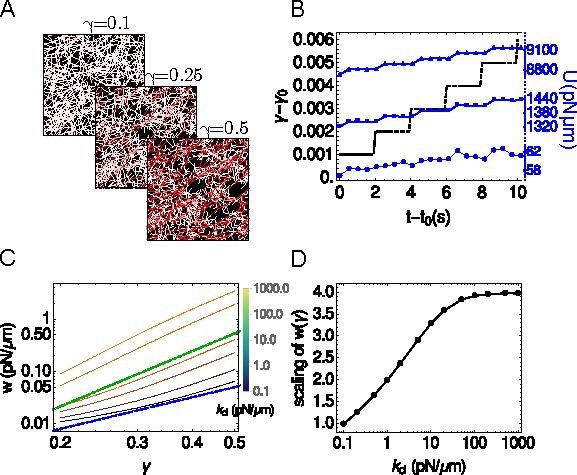
\includegraphics[scale=1.2]{figs/elasticity/shear_result.pdf}
  \caption{%
    \label{fig:stress}%
    Tunable elasticity of crosslinked actin meshes. 
    (A) Snapshots of a strained network ($k_a=k_{cl}=1000$) at $t=0.1s$, 
    $t=0.25s$ and $t=0.5s$. Color indicates stretching energy on each link, with
    white being the lowest and red being the highest. 
    (B) The potential energy of the network as a function of time shown at
    different strains $\gamma_0=0.1$ (circles) $\gamma_0=0.25$ (squares) and
    $\gamma_0=0.4$ (triangles) where $t_0=\gamma_0\times 1s$. Black dashed line
    shows the strain protocol.   
    (C) Strain energy density ($w=U/area$) for various values of crosslinker
    stiffness $k_{cl}$. Blue dashed line indicates expected behavior for a 
    linearly elastic solid $w\propto \gamma^2$ and green dashed line indicates
    strain stiffening behavior of $w\propto \gamma^{3.5}$ as expected 
    for semiflexible polymer networks\cite{gardel2004,lin2010}.
   (D) Power law exponent of $w(\gamma)$, evaluated via least squares fit to
   $ln(\gamma)$ vs $ln(w)$. 
  }
\end{figure}
\subsection{Modulating ensemble motor behavior}
While the force dependent detachment and speed of an individual myosin motor is
a model input (Methods) the ensemble behavior of many motors could provide
a benchmark that the simulation is capable of reproducing dynamics observed in 
actin motility assays \cite{riveline1998, walcott2012}. In a classical motility
assay experiment, a layer of myosin is adhered to a plate, and actin filaments
are placed on top of the motoros. Because the myosin cannot diffuse, they
instead slide the actin filament across the assay. Although this experiment
typically involves single myosin heads, and not myosin minifilaments, we believe
that functionally the situations would be equivalent, with the substitution that
each model motor head approximates the activity of dozens of single molecule
myosin heads. Previous experiments \cite{harris1993, umemoto1990} have reported
a nonlinear dependance of the speed of an actin filament across the assay on the
concentration of myosin, the length of the actin filament, and the concentration
of ATP in the sample. By allowing filaments to interact with more motors, one
can monotonically increase the filament speed to a constant value.
\par
To explore the dynamics of this assay, we randomly distributed motors on a
$(50\mu m)^2$ periodic simulation cell and tethered one head of each motor to
its initial position. Filaments were then introduced in the simulation cell and 
allowed to interact with the free motor heads. The strength of motor-filament
interactions was manipulated in three ways: by varying the motor concentration
$\rho_m$, the filament contour length $L$, and the duty ratio $r_D =k_m^{on}/(k_m^{on}+k_m^{off})$. 
The results are shown in \Cref{fig:motility}, where we have used the
dimensionless control parameter $\mathcal{M} = \rho_m L^2 r_D$ representing the
average number of bound motor heads, to tune filament motility.
\par
Our findings are qualitatively similar to the previously reported experimental 
results. At low $\mathcal{M}$, i.e., low motor density, filament length and duty
ratio, transverse filament fluctuations dominate over longitudinal motion as
the filament is not being propelled by motors faster than diffusion
(\Cref{fig:motility}B). However, as $\mathcal{M}$ is increased, longitudinal
motion dominates. This can be inferred from the dependence of the mean squared
displacement, plotted in \Cref{fig:motility}(D), where low $\mathcal{M}$ 
yields diffusive behavior with an $\langle r^2 \rangle \propto t$, and the
motion becomes ballistic with $\langle r^2\rangle\propto t^2$ as $\mathcal{M}$ 
approaches $100$. The longitudinal speed of the filament plateaus at
$v_{||}\approx 1\mu m/s$ which is the average unloaded speed of a single motor 
head\cite{kron1986}. \Cref{fig:motility}(C) shows that aside from being
propelled, filaments are also buckled in the presence of a large number of
motors, as filament strain, defined as
\begin{equation} 
  \Delta s = \left(1 - {|r_{15}-r_0|\over\sum_{i=1}^{15}{|r_i-r_{i-1}|}}\right) 
  \label{eqn:fil_strain}
\end{equation} 
where $r_i$ is the position of the $i^{th}$ bead on a filament, increases with 
increasing $\rho_m L^2 r_D$.
Although there are no explicit crosslinkers, at a high enough concentration, 
motors near the barbed end of a filament will pin the filaments for a short 
time, and induce buckling the same way crosslinkers do in contractile networks, 
similar to the effects observed in experiment \cite{schaller2010}.
\begin{figure}[H] 
    \centering
    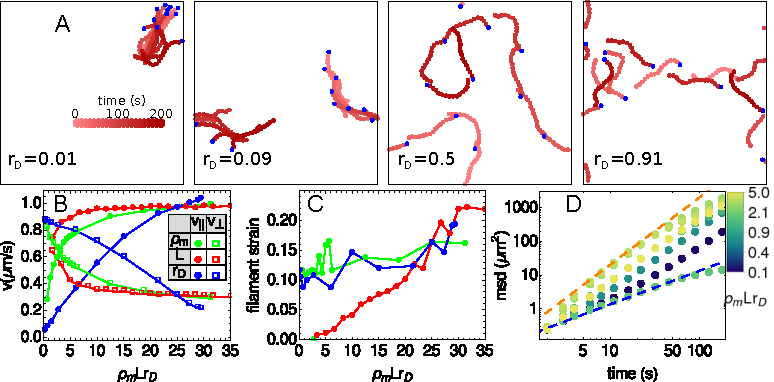
\includegraphics[scale=1.2]{figs/motility/mot_fig.pdf}
  \caption{%
  \label{fig:motility}%
  Driving filament motion by increasing the duty ratio of motors in a motility assay. 
  (A) Position of a filament for $\rho_m = 10\mu m^{-2}$ and $L = 16\mu m$ for
  different values of the duty ratio. White filament is the configuration at
  $t=0$ and dark red represents $t=90s$. Blue dot marks the barbed end of
  filaments.  
  (B) Filament speed decomposed into longitudinal and transverse components. 
  Green: $\rho$ variable, $L=15\mu m$, $r_D=0.95$; Red:
  $\rho_m=4\mu m^{-2}$, $L$ variable, $r_D=0.95$; Blue: $\rho_m = 10\mu m^{-2}$,
  $L=15\mu m$, $r_D$ variable.  
  (C) Filament strain (\Cref{eqn:fil_strain}) as a function of
  dimensionless parameter $\mathcal{M}$.
  (D) Mean squared displacement for various values of $\mathcal{M}$. Blue dashed 
  line has slope $1$ (diffusive) and red dashed line has slope $2$ (ballistic).
 }
\end{figure}
\section{Discussion}
The goal of this paper is to introduce a framework that could accurately and efficiently simulate active networks of F-actin,
myosin, and crosslinker proteins to explore the various structural phases that this system can produce. In doing so, we
have shown that our model passes a series of tests. We use a widely tunable semiflexible polymer model, that
reproduces experimental and theoretical predictions of spatiotemporal fluctuations. We have reproduced the strain stiffening
behaviors observed in experimental assays, and shown how their stiffness could be related to the relative energy
contributions of filaments and crosslinkers. We have qualitatively reproduced sliding filament assays and predicted
crossover points between transversely diffusive and longitudinally precessive motion. 
\par
While this model is thorough in what it aims to simulate it is limited by a few experimental observations that are
currently not implemented. First, the structure of myosin minifilaments is significantly more complex than a two headed
spring. As mentioned, these minifilaments have dozens of heads, which allows them to walk along multiple filaments and
could result in subdiffusive behavior \cite{scholz2016} and significantly increase local network elasticity
\cite{murrellTalk}.
Another limitation of our system is that the actin filaments are static, and will not polymerize, depolymerize or
sever. Within actomyosin assays it is clear that recycling of actin monomers and to a lesser degree, filament severing 
plays an important role in contraction\cite{murrell2012}. Within the cytoskeleton, actin treadmilling is also important
for shape production. Additionally, these simulations are run in $2D$ and without steric interactions, and
dimensionality and volume exclusion may play important roles. While we intend to address and investigate these limitations in future
works, we believe that the successful benchmarking of the simulation at various levels is a significant argument in favor of the
current setup.
\par 
Separately we address a number of possible actomyosin networks that include collective behavior 
and show that we can effectively explore them using our model \cite{freedman2016,stam2016}.
We believe this simulation can shed light on other active polymer assemblies as well,
such as microtubule-kinesin-dynein networks, and that it can help 
elucidate the coupling between microscopic machinery and the biological scaffold 
that comprises the active cytoskeleton. Since the model is parameterized using many 
experimentally manipulateable variables, we also hope that this simulation can be used
by experimentalists to efficiently zero in on biologically relevant and structurally interesting
polymer network phases. 
We believe this simulation can also be used to design biologically-based active
materials and guide our understanding a variety of systems outside the 
cytoskeleton that involve collective dynamics and self-assembly.
\section{Acknowledgements}  
We thank M. Gardel, J. Weare, C. Matthews, F. Nedelec, F.C. Mackintosh, and M. Murrell for helpful conversations. 
This research was supported in part by the
University of Chicago Materials Research Science and Engineering Center
(NSF Grant No. 1420709). S.L.F. was supported by the DoD
through the NDSEG Program. G.M.H. was supported by an NIH Ruth L. Kirschstein
NRSA award (1F32GM113415-01).
\bibliography{actosim}
\bibliographystyle{unsrt}

\beginsupplement
\begin{table}
  \caption{Parameter Values}
  \centering
  \begin{tabular}{|C{2cm}|L{7cm}|C{2cm}|C{2cm}|C{2cm}|}
    \hline\hline
    Symbol & Description (units) [ref] & $L_p$ & Shear & Motility Assay \\
    \hline
    &\bf{Actin Filaments}& & & \\
    \hline
    $N_B$ & Number of beads & $21-201$ & $16$ & $16$ \\
    $l_a$ & Link Rest Length ($\mu m$)\cite{odijk1983}& $1$ & $1$ &$1$\\
    $k_a$ & Stretching Force Constant ($pN/\mu m$) & $0.01-10$ & $10$ & $1$ \\
    $\kappa_B$ & Bending Modulus ($pN\mu m^2$)\cite{ott1993} & $0.002-5 $ & $0.08$ & $0.08$ \\
    \hline
    &\bf{Myosin Minifilaments}& & &\\
    \hline
    $l_m$ & Rest Length ($\mu m$)\cite{niederman1975} & n/a & n/a & 0.5 \\
    $k_m$ & Stiffness ($pN/\mu m$)& n/a & n/a & $1$ \\
    $k^{on}_m$ & Attachment rate at distance $r=0$ ($s^{-1}$)& n/a & n/a &$2-4000$ \\
    $k^{off}_m$ & Unloaded head detachment rate ($s^{-1}$)& n/a & n/a & $200$ \\
    $k^{end}_m$ & Unloaded head detachment rate at the barbed end of the filament ($s^{-1}$)& n/a & n/a &$2000$ \\
    $x_m$ & characteristic bond length ($\mu m$) \cite{stam2015}& n/a & n/a & $0.0004$\\
    $v_0$ & Unloaded speed ($\mu m/s$) \cite{kron1986}&  n/a & n/a & $1$ \\
    $F_s$ & Stall force of myosin ($pN$)\cite{veigel2003}& n/a & n/a & $3.85$ \\
    \hline
    &\bf{Crosslinkers} & & & \\
    \hline
    $l_{cl}$& Rest Length (Filamin) ($\mu m$)\cite{ferrer2008} & n/a &$0.150$ &n/a\\
    $k_{cl}$ & Stiffness ($pN/\mu m$)& n/a & $1,10$ & n/a\\
    $k^{on}_{cl}$ & Attachment rate at distance $r=0$ ($s^{-1}$)& n/a & $10^6,10^5$ &n/a \\
    $k^{off}_{cl}$ & Unloaded head detachment rate ($s^{-1}$)& n/a & 0 & n/a\\
    $x_{cl}$& characteristic bond length ($\mu m$) & n/a & $0.0004$ & $0.0004$ \\
    \hline
    &\bf{Environment} & & & \\
    \hline
    $dt$ & Dynamics timestep (s) & $10^{-4}$ & $10^{-6},10^{-5}$ &$2.5\times10^{-4}$ \\
    $T_F$& total simulated time (s) & $100$ & $0.5$ & $100$ \\
    $X$, $Y$ & Length and width of assay ($\mu m$)& n/a & $75$ & $50$ \\
    $r_c$ & Mesh (actomyosin binding site) size ($\mu m$) & $n/a$ & $0.2 $ & $0.2 $\\
    $T$ & $k_B$ * Temperature ($pN\mu m$)& $0.004$ & $0.004$& $0.004$\\
    $\nu$ & Dynamic viscosity ($mg/(\mu m s)$) & $0.001$& $0.001$& $0.001$\\
    $\gamma$ & Strain (\%) \cite{stricker2010}& n/a& $0.001$&n/a\\
    $t_{relax}$ & Amount of time between sequential strains (s)& n/a& $0.001$ &n/a\\
    \hline
  \end{tabular}
  \label{tab:params}
\end{table}
\end{document}
